\documentclass[10pt,a4paper]{extarticle}
\usepackage[margin=1in]{geometry}
\usepackage[utf8]{inputenc}
\usepackage[IL2]{fontenc}
\usepackage[czech]{babel}
\usepackage{microtype}
\usepackage{amssymb}
\usepackage{amsthm}
\usepackage{amsmath}
\usepackage{xcolor}
\usepackage{graphicx}
\usepackage{wasysym}

\usepackage[inline]{enumitem}


\newtheorem*{poz}{Pozorování}

\theoremstyle{definition}
\newtheorem*{uloha}{\atr Úloha}
\newtheorem*{bonus}{Bonus}
\newtheorem*{defn}{Definice}

\pagestyle{empty}

\def\atr{}
\def\basic{\def\atr{\llap{\mdseries$\sun$ }\gdef\atr{}}}

\mathcode`\,="013B

\begin{document}

\section*{Řešení úlohy s polokoulí}


\begin{uloha}
Bruno v laboratoři naklonil těleso $\mathfrak T$ plné kyseliny o $30^\circ$, čímž se z něj část kyseliny vylila. Určete, jaký objem kyseliny v $\mathfrak T$ zůstal, pokud $\mathfrak T$ je
polokoule o poloměru $1$ (otočená plochou stranou nahoru).
\end{uloha}

\begin{proof}[Řešení]
Nákres situace:
\[ 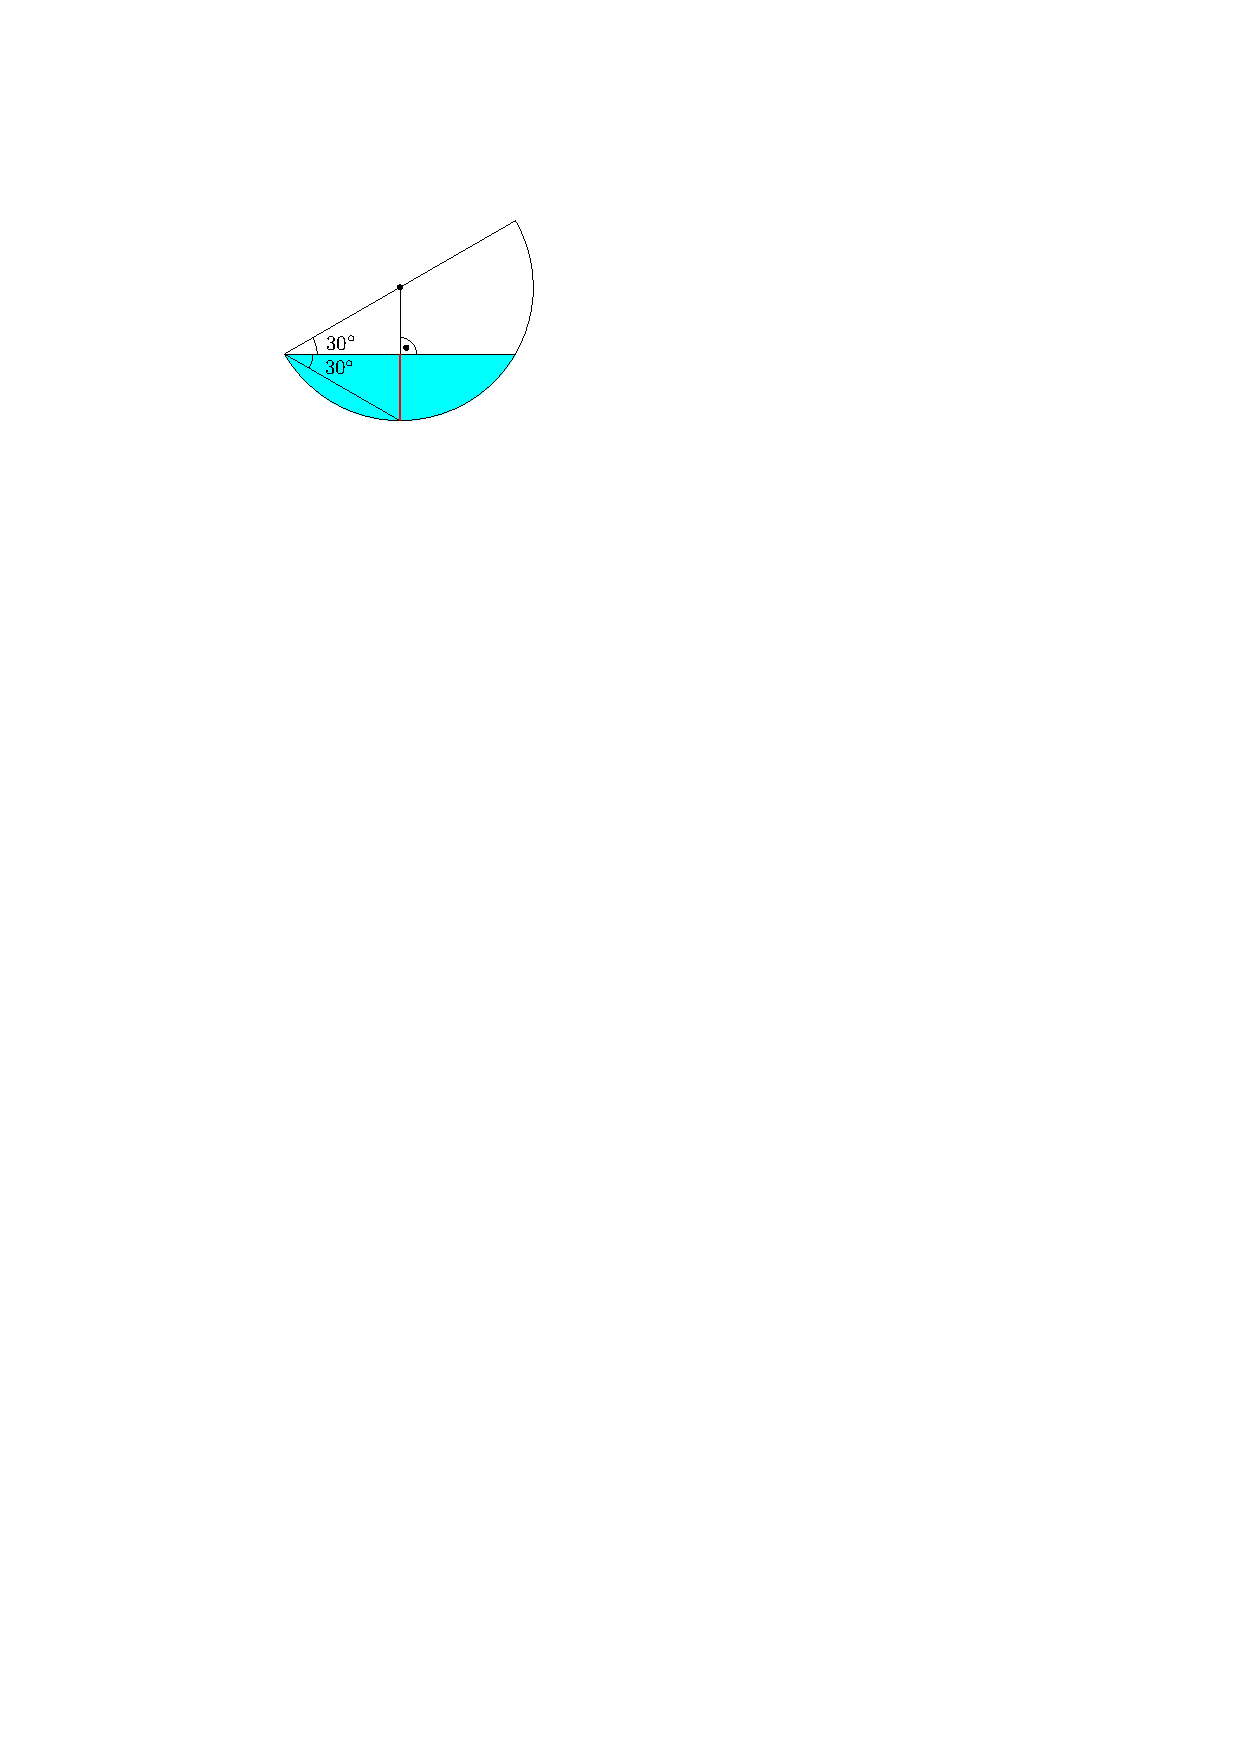
\includegraphics{otoceni_polokoule.pdf} \]
Stačí nám spočítat, jaká bude výška příslušné úseče. V tomto konkrétním případě ($30^\circ$) to bude polovina poloměru, jak je patrné z obrázku (vznikne tam rovnostranný trojúhelník). Stačí tedy již jen dosadit do vzorce pro objem úseče $r = 1$, $v = \frac12$:
\[ V = \frac\pi3 \left(\frac12\right)^2 \left(3 - \frac12\right) = \frac{5}{24}\pi \doteq 0,6545. \]

V méně speciálním případě, např. $40^\circ$, je postup obdobný:
\[ 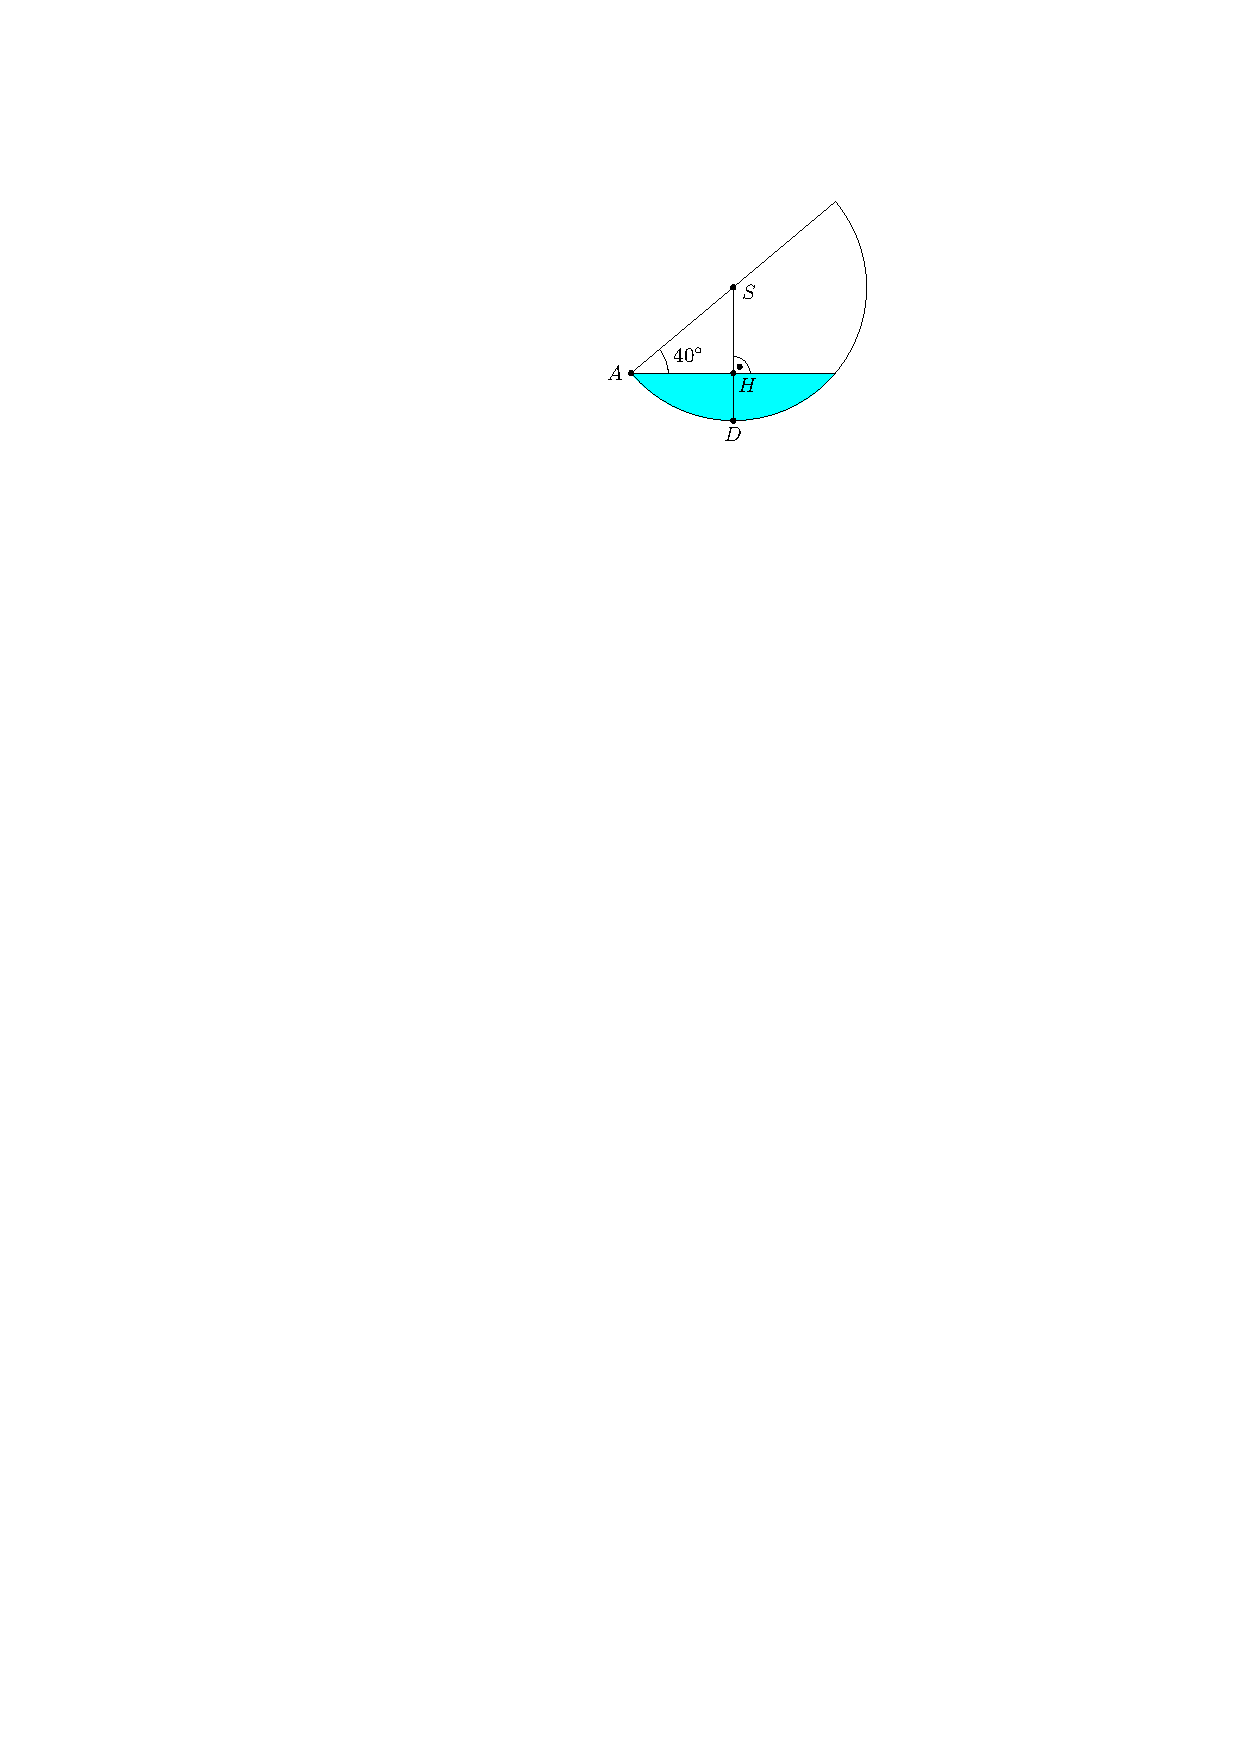
\includegraphics{otoceni_polokoule_mene.pdf} \]
Zajímá nás $|HD|$, což spočteme jako rozdíl $|SD| - |SH|$, přičemž $|SD|$ je poloměr, tj. 1, a $|SH| = \sin 40^\circ$ s~využitím pravoúhlého trojúhelníka $AHS$ (opět $|AS| = 1$). Do vzorce pro objem úseče tedy dosadíme $r = 1$, $v = 1 - \sin 40^\circ$. Vyjde přibližně 0,3531.
\end{proof}


\end{document}